\onehalfspacing
\section{Empirical Methodology}\label{sec:methodology}
\vspace{-0.3cm}
As briefly discussed in \textbf{\hyperref[sec:dependent]{Subsection 3.3}}, this thesis employs ... :

introducing TikZ:

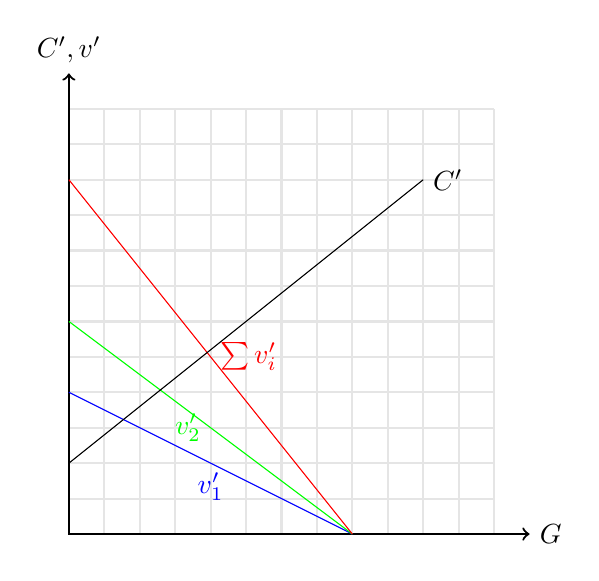
\begin{tikzpicture}[scale = 0.9]
		\draw[thick, step = 0.5cm, color = gray!20] (0,0) grid (6,6);
		\draw[thick, step = 0.5cm, color = gray!20, opacity = 0.3] (0,0) grid (6,6);
		\draw [<->,thick] (0,6.5) node (yaxis) [above] {$C' , v'$}
		|- (6.5,0) node (xaxis) [right] {$G$};
		\draw[blue] (0,2) -- node[below]{$v^{\prime}_1$} (4,0) ;
		\draw[green] (0,3) -- node[below, left]{$v^{\prime}_2$} (4,0);
		\draw[red]  (0,5) -- node[above, right]{$\sum v^{\prime}_i$}(4,0) ;
		\draw[black] (0,1) -- (5,5) node[right]{$C'$};
	\end{tikzpicture}


\subsection{Model 1}\label{sec:model1}
\vspace{-0.3cm}
\justifying
In the first empirical model, I define $Y_{it}$ as the dependent variable for individual $i$ at time $t$. For this model, the dependent variables are the \textit{Dep Var 1}, ... :

\vspace{-0.3cm}
\begin{equation}
Y_{it} = \alpha_i + \beta_1\text{DepVar1}_{it} + \beta'X'_{it} + \epsilon_{it}
\tag{1}
\end{equation}

\noindent
Moreover, the model incorporates the vector $X'_{it}$, which includes control variables to improve the precision of the estimates ... 


\subsection{Model 2}\label{sec:model2}
\vspace{-0.3cm}
\justifying
Analog to above...




% End of this section.
